\chapter{Match+Action Processing Pipeline}
\label{chap:matchActionProcessing}

\begin{chapterintro}
% Tato kapitola bude obsahovat zakladni architekturu procesni pipeliny
In this chapter, we introduce results of our research regarding the Match+Action processing pipeline with 
details about transformation algorithm and generated architecture. We introduce mapping from P4 language to 
Match+Action groups, Match+Action tables and Match+Action routers which are the main building blocks of our pipeline.
We also provide more details about usage of HLS which can be beneficially used for easy extension of available actions. 
\end{chapterintro}

\section{Main Building Blocks}
% Tady se napise, jak se z te P4 dostane ta pipelina a identifikuji se zakladni bloky
% 1) Plne tabulky s akcnima blokama
% 2) Routovaci tabulky
% Dale budeme psat, jak se identifikuje kontrolni program a jak se zahrne do zakladnich bloku.

The main building block of our architecture is the \emph{Match+Action group} which was briefly introduced in 
Sec.~\ref{sec:architectureOfProcessingPipeline}. We also introduced the idea for mapping of P4 
language constructs to Match+Action pipeline elements in Sec.~\ref{sec:mappingP4ToProcessingPipeline}.
As we notice before, each \emph{Match+Action group} represents one \emph{control program} from 
translated P4 source and it contains one or more pipeline elements (tables or routers).
Such group of building blocks is used for implementation of complex 
processing of parsed data. The following text introduces detailed architecture of proposed blocks.

We noticed that elementary building block is the \emph{Match+Action table} which implements functionality
of protocol field processing based on user defined P4 program. 
The engine performs three operations: (1)~searching for the most suitable operation regarding
to used headers and metadata, (2)~computation of next used Match+Action element address and (3)~execution of selected 
action on headers and metadata. During our research, we identified two types of pipeline engines:
\begin{enumerate}
    \item \textit{Match+Action table}
    \item \textit{Match+Action router}
\end{enumerate}

The first type, full \textit{Match+Action table}, is the engine with full functionality which was described in
previous text. It contains engines for searching of the most suitable action (i.e., the match engine), engines for computation of next table address and
engines for execution of selected action on incoming headers and metadata. We provide more details about this Match+Action block in 
Sec.~\ref{sec:matchActionTables}.

The second type, \textit{Match+Action router}, is the engine with limited functionality. It just computes
the next table or router address from incoming headers and metadata values. Such node allows us to implement (or represent) 
the conditional selection of next table or router address without instantiation of search and action engines. 
In other words, it allows us to map the \textit{if-else} statement more directly from P4 source to Match+Action processing pipeline.
We provide more details about this engine in Sec.~\ref{sec:matchActionRouters}. 

The architecture of the Match+Action processing pipeline is published in this \thesis{} because it is the latest result of our research.
We start the introduction of our approach with description of mapping from P4's \emph{control program} to pipeline of Match+Action elements.

\subsection{Control Program}
\label{sec:matchActionProgram}
% Dale popsat jak do toho zakomponovat ten obsluzny program, kazdy blok rozhodne co bude dal.
% Take, ze ten kontrolni program definuje vsechno ostatni, jak zjistim zapojeni, jak ho vygeneruju
We briefly introduced the structure of \emph{control program} in Sec.~\ref{sec:mappingControlToMaGroup}. 
It indirectly defines a sequence of Match+Action elements (tables and routers) and we can see it as an imperative program. 
The program may apply tables, call other control flow programs or test conditions. 
The execution of a table is invoked by the \textit{apply} statement and it has four modes of operation (more information in \cite{p4languagespec}):
(1)~sequential, (2)~selection based on executed action, (3)~hit/miss check and (4)~conditional selection based on \textit{if-else} statement.
The first mode, sequential, is the unconditional movement to the next table or router in control flow.
The second mode is the conditional selection based on executed action in current table.
The third mode performs selection of next pipeline element based on hit/miss event in actually used table.
The test condition is classic \textit{if-else} statement which is similar to C language conventions.
Examples of each mode are given below this text.

\begin{Verbatim}[fontsize=\small]
control Ingress {
    // Sequential mode
    apply(table1);
    apply(table2);
    
    // Action selection mode
    apply(table3) {
        action1 : {apply(table4)};
        action2 : {apply(table5)};
        default : {apply(table6)};
    }
    
    // Hit/miss check     
    apply(table7) {
        hit     : {table8);}
        miss    : {table9};}
    }

    // Test condition
    if(valid(ipv4) and ipv4.ttl < 42){
        apply(table10);
    }
}
\end{Verbatim}

The above example introduces the program called \textit{Ingress}, including ten tables. The fist three tables are used in sequential manner.
Our program follows by invocation of table regarding to executed action in \textit{table3}. The example also introduces the usage of 
default rule for coverage of situation without any matched action. The control flow of our program continues with invocation of \textit{table7}. 
Next tables, \textit{table8} and \textit{table9}, are invoked based on hit/miss result in \textit{table7}. 
Finally, our example introduces a simple test condition for IPv4 header. The header is checked for validity and value of \textit{ttl}
field. The \textit{table10} is used if both parts of the condition are satisfied.

As you can see from provided example, the \emph{control program} describes the structure of the \emph{Match+Action group} in terms
of used Match+Action elements (i.e., used tables and routers). Therefore, our main task is to use the description of \emph{control program} 
and generate the structure of Match+Action pipeline. We introduce details of this transformation in next section of this text.

\subsubsection{Generation of the Pipeline Structure from Control Program}
\label{sec:generateOfThePipelineStructureFromControlProgram}
% Tady se popise cast o tranformaci kontorlniho programu do struktury pipeliny
The main idea of the transformation is similar to identification of parser's structure which was introduced in 
Sec.~\ref{sec:overviewOfHfeM2}. 
We described a \textit{Parser Graph Representation}\,(PGR) as an input to our
transformation algorithm. The PGR is an oriented acyclic graph which represents relations between protocols. 
After that, we used the \textit{depth-first-search} algorithm for identification of Protocol Analyzer position in generated parser pipeline. 
The proposed idea can be reused for identification of the Match+Action pipeline structure. 
However, we cannot reuse the graph because all nodes of PGR have the same type (i.e., each node represents the Protocol Analyzer block).
The \emph{Match+Action group} contains two types of blocks: \emph{Match+Action tables} and \emph{Match+Action routers}.

\begin{figure}[ht]
	\centering
	\includegraphics[width=0.9\textwidth]{chapters/pic/control-program-graph}
	\caption{Graph of the control program from the example.}
	\label{fig:controlProgramGraph}
\end{figure}

The new tree structure reflects the previous need. Each node of refined graph represents one Match+Action table or router and each 
transition represents the next used Match+Action element. 
Condition of each transition is inferred from P4's \emph{control program}. 
The refined structure also defines a common root node which is used as a starting point for processing of different \emph{control program}s 
using one algorithm. 
All remaining properties of the refined structure stay the same (i.e., the graph is oriented  and acyclic). 
This structure is built using the \textit{depth-first-search}\,(DFS). 
The example of refined tree structure is shown in Fig.~\ref{fig:controlProgramGraph}.

Generation of the Match+Action pipeline uses the refined tree structure as an input. 
The main problem is the same as generation of parser's structure from PGR representation. 
Therefore, we reuse the algorithm for identification of the longest path to each node in refined graph.
That is, we use the Alg.~\ref{alg:longest} from Sec.~\ref{sec:parserTransformation}. 
The result of the algorithm is shown in Fig.~\ref{fig:controlProgramGraph} and the longest path to each node is expressed by a number.
Finally, all nodes are connected in any non-decreasing order. The example of such pipeline is shown in Fig.~\ref{fig:controlProgramPipeline}.
The Match+Action engine does nothing if it is not selected (i.e., it passes input to output without any change). The structure of Match+Action
pipeline follows architectures of parser and deparser. That is, each engine can be followed by optional pipeline for tuning of final frequency or 
latency. We introduce the architecture and transformation from P4 to Match+Action pipeline in following text.

\begin{figure}[h]
    \centering
    \includegraphics[width=0.9\textwidth]{chapters/pic/control-program-pipeline}
    \caption{Generated Match+Action pipeline from the example.}
    \label{fig:controlProgramPipeline}
\end{figure}

\subsection{Match+Action Routers}
\label{sec:matchActionRouters}
% Popis router
The \textit{Match+Action router} is the second engine which is used in our architecture. As we noticed before, it is engine with limited functionality because
it is used for implementation of \textit{if-else} conditions. 
The engine computes the next table or router address from incoming header and metadata fields. 
Therefore, the engine does not need to implement any match or action sub-engine. 

The \textit{if-else} condition can contain field or header references, valid operator (used for detection of header validity), binary operators
(including arithmetic and logic operations), unary and relation operators (e.g., less than, equal, less or equal, and so on).  
Therefore, our engine has to support a variety of common operations for selection of the next table or router address in pipeline. 

\begin{figure}[ht]
    \centering
    \includegraphics[scale=0.9]{chapters/pic/match-action-router-architecture}
    \caption{Architecture of Match+Action router.}
    \label{fig:architectureMatchActionRouter}
\end{figure}

The architecture of Match+Action router is shown in Fig.~\ref{fig:architectureMatchActionRouter}. 
The proposed interface is common for both engines (router and table) and it is also used for easy connection between engines. 
This interface provides the input information necessary to process one single condition. That is: (1)~protocol headers, 
(2)~incoming metadata and (3)~control path signals (including table or router address, drop control, next/valid signalization, and so on). 
The output information includes (4)~original protocol headers, (5)~original metadata and (6)~output control path. The last mentioned 
output is modified by the router engine because the control path contains the address of next element (table or router).

Each Match+Action router contains \textit{Next Address Logic} block. The block is generated from scratch and it is configured with address of the 
router (i.e., it is configured with address in the pipeline).
This information is used for activation of the engine which leads to computation of the next element address. 
Any headers, metadata or control signals aren't modified if address 
differs from the configured one. The behavior of \textit{Next Address Logic} block depends on condition in the \textit{if-else} statement.
The translation of this condition is based on \textit{Expression Tree} which is translated into HDL language (VHDL in our case) by 
\textit{in-order} tree traversal. An example of this process is shown in Fig.~\ref{fig:matchActionRouterNextAddressExample}. 
The example also shows the parallel nature of HDL language because all lines of provided code are executed at the same time.

\begin{figure}[ht]
    \centering
    \includegraphics[width=\textwidth]{chapters/pic/match-action-router-next-address-logic-example}
    \caption{The example of transformation from P4 to the \textit{Next Address Logic} block.}
    \label{fig:matchActionRouterNextAddressExample}
\end{figure}

The example introduces the process of transformation for the condition from previous section. Firstly, each condition is transformed 
to the \textit{Expression Tree} where each node represents an operation (arithmetic, logic or relation) and each leaf represents a value, 
referenced header or field. 
Secondly, we use the \textit{in-order} tree traversal for generation of the VHDL representation. 
The generated code reflects proposed functionality needs.
It selects the next table address if generated condition was satisfied and engine was selected 
(i.e., the IN\_TABLE\_ADDRESS value equals to the address which was assigned to the engine during translation of P4 source). 
The input address is transferred to the output unchanged if the engine wasn't selected.

\subsection{Math+Action Tables}
\label{sec:matchActionTables}
% Popis tabulek, jak implementovat hledani atd.
The \textit{Match+Action table} is important engine of Match+Action pipeline because it implements match and action engines for further processing of header
and metadata fields. The engine performs three operations: (1)~searching for the most suitable action, (2)~computation of next used
Match+Action router or table address and (3)~invocation of selected action on header and metadata fields. 

Behavior of Match+Action table engine is inferred from the following P4 language constructs: Match+Action Table definition, Action definition and
Protocol Header definition. The first language construct is used for specification of required match fields (including matching algorithms)
and supported actions in this engine. The structure of incoming header and metadata fields is described by Protocol Header definition. 
Finally, the behavior of supported actions is described by Action definitions. There are two types of actions --- user defined and primitive.
The user defined actions have a list of required parameters and unique name across the P4 program. Each user defined action contains calls of 
primitive or other user defined actions. Therefore, we can implement quite complex operations which can be executed on incoming header and metadata
fields. 
The list of primitive actions includes modification of header fields, insertion or deletion of protocols from packet, 
arithmetic operations on incoming data, and so on.  
The behavior and list of primitive actions is defined in P4 language specification \cite{p4languagespec}. 

\begin{figure}[ht]
    \centering
    \includegraphics[width=\textwidth]{chapters/pic/match-action-table-architecture}
    \caption{Architecture of Match+Action table.}
    \label{fig:matchActionTableArchitecture}
\end{figure}

The architecture of Match+Action table engine is shown in Fig.~\ref{fig:matchActionTableArchitecture}.
Each pipeline engine uses the interface from Sec.~\ref{sec:matchActionRouters}. 
This interface provides the input information necessary to process a table request. 
That is: (1)~input protocol headers, (2)~input metadata,(3)~control path signals (including table or router address, drop control, and so on)
and (4)~configuration interface which is used for filling of rules with corresponding actions and parameters. 
The output interface includes (5)~protocol headers, (6)~metadata and (7)~control path signals. 
The output headers are changed based on selected action. 
All input protocol headers and metadata fields are stored in auxiliary FIFO memories. 
These memories are used to cover the initial latency of \textit{Search engine}. 
Examined protocol headers and metadata fields are passed to \textit{Search engine} which is responsible for searching for the most suitable 
action. The set of used protocol header and metadata fields is inferred from P4's Match+Action Table declaration (\textit{reads} statement). 
The output of the engine provides information necessary for processing in \textit{Action engine} 
(i.e., selected action and parameters) and computation of the next table or router address (based on executed action and hit/miss information). 
All input blocks (FIFO memories and \textit{Search engine}) are controlled by the \textit{Ready\&Next} engine. 
The engine is configured with address of the Match+Action table during translation of P4 source code. 
The configured address is used for activation of Match+Action table if the input address equals to the expected one.
The \textit{Action engine} accepts packet control information (drop contol for example), protocol headers and metadata (from FIFO memories), 
and selected action (including parameters). 
This engine is generated from scratch for each \textit{Match+Action table} in design. 
The behavior of user actions is inferred from P4's Action definitions. 
We describe the \textit{Action engine} in Sec.~\ref{sec:actionEngine}. 
Finally, the last output block (SYNC) is used for synchronization of results from \textit{Action engine} and FIFO to output.

We identified three types of blocks from proposed architecture: 
(1)~Configured (grey color), (2)~Fully table specific (blue color), and (3)~Mixed (red color).
The first group is general enough for usage in all \textit{Match+Action tables}, only with different parameter settings like 
data width, assigned address in pipeline, and so on. 
The second group of blocks, table specific, are fully generated regarding to P4's Match+Action Table declaration. 
In our case, we fully generate the \textit{Next Address Logic} and \textit{Action engine}. 
The \textit{Action engine} and its generation was briefly described in previous text and we provide more details in 
Sec.~\ref{sec:actionEngine}.
Finally, the third type of blocks is the example of mixed architecture where some parts are fully generated and some parts are configured 
by parameters during translation.

Generation of \textit{Next Address Logic} is quite straightforward because P4 language defines three modes for selection of next address 
(action based, sequential and hit/miss check). Therefore, the generation of the code is easier because we don't need to deal with
complex structures of test conditions (\textit{if-else} statements). The logic of HDL code generation stays similar for different implementations
of \textit{Match+Action table}. 
Main differences are in selection of table or router addresses based on executed action or current hit/miss result in \textit{Search engine}.
The example of transformation, including the structure of generated VHDL code, is provided in Fig.~\ref{fig:matchActionTableNextAddressLogicExample}.

The \textit{Search engine} is used for mapping of incoming protocol and metadata header fields to used actions and parameters. 
The structure of this block can be complex because P4 language allows usage of different match algorithms for each used protocol or 
metadata field. We introduce the architecture of this block in following section.

\begin{figure}[h]
    \centering
    \includegraphics[width=\textwidth]{chapters/pic/match-action-table-next-address-logic-example}
    \caption{The example of transformation from P4 to the \textit{Next Address Logic} block.}
    \label{fig:matchActionTableNextAddressLogicExample}
\end{figure}

\subsubsection{Search engine}
\label{subsubsec:matchActionSearchEngine}
The P4's Table specification defines a list of used 
protocol header fields together with matching algorithm. Current version of the language supports following algorithms:
range, ternary, Longest Prefix Match (LPM), exact and header validity checking. 
%We introduced current classification approaches in Sec.~\ref{sec:classification}.

Design of general classification approach (suitable for P4) is out of scope of this thesis. 
Therefore, we utilize a TCAM because
it implements exact, ternary and range match (after some changes \cite{MeinersClasssificationBook}).
Each row of TCAM contains one rule. In this approach, all used protocol headers and metadata are concatenated to create one wide lookup key to TCAM. 
Returned vector contains information about all matched rows (in one-hot encoding).
The vector is passed to the priority encoder which identifies the address of most suitable rule. The computed address is used as an input to rule memory 
which contains data with encoded action and parameters. 
We also identify the common interface for \textit{Search engine}
which is used for communication with neighboring blocks (see Fig.~\ref{fig:matchActionTableArchitecture}).
That is: (1)~used protocol headers, (2)~used metadata, (3)~search engine control (VLD/NEXT signaling) and (4)~interface for configuration from software. 
The output includes information necessary for computation of the next table address (based on hit/miss check or executed action). 
The \textit{Search engine} is also equipped with a special configuration bus which is used for filling of rules with corresponding action and parameters.
Finally,the series of outputs are used for passing of selected actions and parameters to \textit{Action engine}. This interface allows easy
and fast replacement with more advanced \textit{Search engines}. 

\subsection{Action Engine}
\label{sec:actionEngine}
% Popis akci + nejak obecne jak je z tech popisu dostat
The \textit{Action engine} performs operations on packet control information (drop control for example) and incoming metadata or protocol header fields.
The outputs of this block are modified protocol or metadata fields based on selected action from \textit{Search engine}.
Supported table actions are provided in P4's Match+Action Table definition (\textit{actions} statement; more details in 
Sec.~\ref{subsubsec:matchActionTableDefinition}).
Each record of \textit{actions} statement is a user defined action with a unique name in P4 program. 
In general, each user defined action is a compound action consisting of primitive and other user defined actions. 
The specification and set of supported primitive actions is defined in P4 language specification \cite{p4languagespec}. 
Therefore, each user defined action can be expressed using a list of primitive actions which are connected together. 
Consequently, we can define the library of all primitive action in HDL and connect together all used actions.
There are two architectural approaches for arrangement of action engines: \textit{serial} or \textit{parallel}.
Brief descriptions of both architectures are provided in Fig.~\ref{fig:basicArchitectures}.

\begin{figure}[t]
    \centering
    \begin{subfigure}[b]{\textwidth}
        \includegraphics[width=\textwidth]{chapters/pic/action-engine-serial}
        \caption{Serial architecture.}
        \label{fig:actionSerial}
    \end{subfigure}
    ~
    \begin{subfigure}[b]{0.85\textwidth}
        \includegraphics[width=\textwidth]{chapters/pic/action-engine-parallel}
        \caption{Parallel architecture.}
        \label{fig:actionParallel}
    \end{subfigure}
    
    \caption{Basic architectures of Action engine.}
    \label{fig:basicArchitectures}
\end{figure}

The first one, serial, is the example of classic architecture for implementation of processing pipeline. This approach is shown
in Fig.~\ref{fig:actionSerial}. It contains two sub-engines --- \textit{action blocks} and \textit{pipelines}. 
The \textit{pipeline} is an optional block which is used for tuning of final latency and consumed resources. 
The most important part is the \textit{Action block} which implements the functionality of processing pipeline. 
Each \textit{Action block} has similar structure and it can be seen from the proposed figure. Firstly, action parameters are parsed in 
\textit{Parameter parser} for easier usage of action parameters in \textit{Action blocks}. 
Finally, the \textit{Action enable logic} is used for controlling of reaction on incoming action value. 
The engine is enabled if the value of action equals to configured value which is assigned to action during translation of the table's P4 source.
Incoming data are transferred through the action block untouched if the value of action differs from the expected one. 
The advantage of this approach is a regular structure which is suitable for generation from abstract description. 
Unfortunately, this architecture is not suitable for latency sensitive applications because data pass through all
action blocks. Therefore, the total latency can be expressed as the sum of all latencies on the path. In our case, 
higher latency leads to higher memory requirements on Payload Buffers.

The second architecture, parallel, is a different approach for arrangement of action blocks. 
This approach is shown in Fig.~\ref{fig:actionParallel}.
The input block of this architecture is the \textit{Distributor}. This block is used for distribution of incoming data to action blocks based on
the value of action from \textit{Search engine}. The \textit{Distributor} block also contains engine for assignment of synchronization tags. 
The synchronization tag is used for selection of output data from action blocks because we need to preserve the order of requests during 
data processing. This approach is suitable for shortening of latency because a request doesn't need to be passed through all action blocks.
The latency for processing of input data depends on actual distribution and usage of action blocks because distributed requests are 
synchronized by \textit{Selection} block. 

From the proposed description of \textit{Action engine} architectures, we rather use the parallel architecture because the processing latency 
depends on distribution of requests. The P4 language defines a fixed set of primitive actions. 
Unfortunately, this limitation is not suitable for future development because we typically need to extend the current action set with new actions 
(e.g., computation of advanced statistics, pattern matching, and so on). The user defined actions can be described using the HLS which
is beneficial for fast development. Moreover, the source code of new action can by provided by administrator, mathematician or security expert.
The next text provides details about usage of HLS in high-speed environment.
The results of our research were verified in SDM \cite{KekelyPusKorenekSDM} project which is actively used for monitoring and protection 
of computer networks. We also demonstrated our research in several network applications 
(NetFlow and non-NetFlow kinds of data processing) which were published in 
\cite{2014hls-instructions,2014sdmcpd-monterey,2014sdmmemincs,kekely2014trade}.

\section{Extending P4 with Non-Standard Actions}
\label{sec:utilizationHlsSdmUpdate}

The parallel architecture of Action engine is similar to \textit{SDM Update} block which is an application specific network processor for
a stateful flow-based network traffic measurement. We introduced this approach in \cite{PusBenacekSDMUpdate}.
The proposed work also introduces usage of HLS in high-speed network environment which helps us with faster development of 
new processing engines. This approach can be also used for extensions beyond P4 language because the set of primitive actions is limited. 
There are situations when we need to support more complex operations which cannot be implemented with actual set of primitive actions. 
There are two possibilities for implementation of new action. The first possibility is to use the HDL language which is the 
most common approach because the architecture and implementation details are under control. As a result, we can get fast and efficient implementation
of new action. However, the development time can be quite high compared the utilization of HLS.
Rather, we can describe new action in C/C++ language and connect it to the existing infrastructure. 
The results of this research was also used by Kekely et al. in \cite{KekelyPusKorenekSdmIeeeTransactionComputerNetworks}.
We demonstrate our approach on \textit{SDM Update} in next section. 
The main proposed ideas can be also used in the case of \textit{Action engine} for implementation of more complex instructions in shorter time.

Software Defined Monitoring (SDM) \cite{KekelyPusKorenekSDM} relies on advanced monitoring tasks implemented in software which is supported by a
configurable hardware accelerator. The monitoring tasks reside in the software and can easily control the level of detail retained 
by the hardware for each flow. This way, the measurement of bulk/uninteresting traffic is offloaded to the hardware, 
while the interesting traffic is processed in the software. SDM enables creation of flexible monitoring systems capable of deep packet
inspection at high throughput.

\subsection{SDM Architecture}
\label{sec:sdm}
SDM consists of two main parts (firmware and software) connected together via PCI Express bus. 
Both parts are tightly coupled together to allow a precise control of the traffic processing on the per-flow basis.
The software part of SDM consists of the controller and monitoring applications. 
The advanced monitoring tasks, such as analysis of application protocols, are performed in the monitoring applications.
The management of the hardware (removing and insertion of the processing rules) is performed in the controller.
The SDM Processor hardware is controlled by instructions stored in the rules.
The instruction tells the hardware what action must be performed for each input packet.
The hardware passes the data to the software in the form of packet metadata (i.e., extracted information from the packet header)
or aggregated flow records (NetFlow for example).
Whole received packet can be also sent to software for deeper analysis. 
Graphical representation of the SDM concept is shown in Fig.~\ref{fig:sdmArchConcept}.
The following text is focused on description of SDM Processor.

\begin{figure}[t]
\centering
\includegraphics[scale=0.57]{chapters/pic/sdm_arch}
\caption{Brief SDM Architecture.}
\label{fig:sdmArchConcept}
\end{figure}

\subsection{SDM Processor Description}
For the scope of this work, the hardware part of SDM is the most interesting.
SDM Processor is conceptually an application specific network processor for a stateful flow-based network traffic measurement.
The main parts of the SDM Processor are  
shown in Fig.~\ref{fig:sdmBrief}. The processing of all incoming packets starts with header
parsing and extraction of interesting metadata in the \textit{Parser} block. 
This prepared data is passed to the \textit{Search} engine which performs lookup in the table of rules 
(these rules are maintained by the software SDM Controller).
If the rule is found, it is sent with the data to the \textit{SDM Update} engine which performs the operation with respect to the passed instruction.
If the rule is not found, default behavior is performed (packet is typically passed to the software for further analysis).

\begin{figure}[b]
\centering
\includegraphics[scale=0.58]{chapters/pic/sdm_update_sch}
\caption{Brief SDM Update architecture and its connection in SDM concept.}
\label{fig:sdmBrief}
\end{figure}

\subsubsection*{Update}
The \textit{SDM Update} engine brings the statefulness to the SDM Processor. 
It manages the flow records --- updates the aggregated data.
It mainly updates the stored values based on the input data and the rule action.
The action for every packet has the address of the record and a specification of the operation
(aggregation type). Update of the record is delimited by two memory operations: read the stored values of
the record and write back the updated values. 
Special type of operation is the export of record values,
possibly followed by clearing the record values in the memory. 

Infrastructure around \emph{Instr x} blocks is designed with respect to easy implementation of new instructions.
Blocks of this generalized environment are shown in Fig.~\ref{fig:sdmBrief}. The main services of this
infrastructure are:

\begin{itemize}
\item Decoding and forwarding of a request to the appropriate processing engine.
\item Memory record reservation (to avoid RAW data hazards).
\item Memory access arbitration.
\item Output synchronization (to preserve the ordering of requests).
\end{itemize}

The idea for fast implementation of new instructions is following:
As a new network monitoring software plugin is installed to SDM, it is accompanied by a description of the most time consuming task in C language.
The task is then synthesized to VHDL and inserted directly to the SDM hardware in the form of a new instruction block. 
The FPGA firmware has to be resynthesized in our system, but the partial dynamic reconfiguration could allow dynamic 
changes of the SDM Processor instruction set in the future.
During the runtime, the SDM controller software installs the processing rules to the hardware.
The hardware then executes the new instruction for each packet of selected flows.

To insert the new instruction engine to the \textit{SDM Update}, the surrounding sub-engines around the instruction blocks stay 
unchanged.
Hence, we implement instruction engines in HLL (C or C++ in our case), perform HLS of this code, connect 
the generated instruction engines and add routing information into the \textit{Instruction Decoder} routing table.
This process of development consumes less time and allows faster implementation of the new hardware accelerated function.
Moreover, final solution is verified during implementation of new accelerated block because modern tools
for HLS require implementation of the testbench file.
After this verification, new engine is easily connected into the existing and tested infrastructure.
As a demonstration, we implement following instructions:
\begin{itemize}
\item The \textbf{Identity (I0)} instruction is used for transformation of input request to the predefined output format.
This engine doesn't perform any update at all, it is rather used for data output synchronization and transformation. The Identity
engine is implemented in VHDL language because it is considered to be the part of the SDM Processor infrastructure.
\item The \textbf{NetFlow (I1)} instruction is used for NetFlow aggregation. It updates the flow start/end timestamp, 
increases packet/byte counters, and performs logical $or$ of TCP flags. NetFlow engine is implemented in both VHDL and C languages for comparison.
\item The \textbf{NetFlow Extended (I2)} instruction demonstrates an easy extension of existing C implementation.
Basic update functionality of this instruction is the same as described in I1. In addition, I2 stores the TCP flags of the first five packets.
This additional information may become very useful for analysis of TCP handshake or for 
detection of network attacks like DoS. The NetFlow Extended engine is implemented in C language with usage of the existing code from I1.   
\item The \textbf{TCP Flag Counters (I3)} instruction is the implementation of non-NetFlow update. 
The instruction performs incrementation of counters of observed TCP flags.
For example, one can see the number of ACK flags transmitted during the whole TCP connection.
Information from this aggregate can be used to support advanced flow analysis \cite{Moore05discriminatorsfor}.
This engine is implemented in C++ language.
\item The \textbf{Timestamp Diff (I4)} instruction is another implementation of non-NetFlow update.
This instruction creates an aggregated record of inter-arrival times of the first eleven flow packets. 
These times are computed with nanosecond precision. 
The engine is implemented in C language. Information from this
aggregated record can be used as a network discriminator for flow-based classification \cite{Moore05discriminatorsfor} 
or for identification of application protocol \cite{Piskac2011DynamicsOfNetworkServices}. 
\end{itemize}

\subsection{Results}
\label{sec:results}
To verify the designed \textit{SDM Update} part of the SDM Processor, we have implemented a prototype of the described architecture. 
We choose the board equipped with Virtex-7 H580T FPGA which is powerful enough for processing of 100\,Gbps traffic \cite{combo-100g}.
The Xilinx Vivado HLS version 2013.2 was used for HLS (C to VHDL).
The Xilinx ISE version 14.6 was used for VHDL to FPGA netlist synthesis.
We have disabled all synthesis optimizations to avoid the register duplication and other modifications that can lead to higher 
frequency but also to higher resource usage. 

The resource usage of the instruction blocks is shown in Tab.~\ref{table:resBaseBlocks}.
We compare the resources of hand-written VHDL code to the HLS based implementation of the I1 instruction.
One can see that the hand-written implementation
occupies less FPGA resources and the final frequency is higher than HLS based solution. 
However, the time needed for VHDL implementation is approximately two times longer than for the solution synthesized from C language. 
The HLS is also very useful for non-HDL programmers because they can create hardware accelerated engine very easily from
the C/C++ source code. 

Tab.~\ref{table:resSdmUpdate} shows the total resource utilization of the whole \textit{SDM Update} engine. 
Each line of this table lists the instructions supported in synthesized engine.
Frequency results from HLS are good enough for processing of the high-speed network traffic.
We consider the minimal frequency of 200\,MHz and the initialization interval of one as the requirement for 100\,Gbps traffic processing.
All synthesized variants of the \textit{SDM Update} meet the frequency requirement for processing of 100\,Gbps traffic. 

\begin{table}[ht]
    \centering
    \begin{tabular}{|l||c|c|c|}
        \hline
        \T{\textbf{Instruction}} & \T{\textbf{Slice Reg}\,[-]} & \T{\textbf{Slice LUT}\,[-]} & \T{\textbf{Frequency\,[MHz]}} \\ \hline\hline
        %RMW Privilege           &             46              &             151             &            404.236            \\ \hline
        %Arbiter                 &             379             &            1129             &            304.614            \\ \hline
        (I0)Identity             &             495             &             504             &            627.559            \\ \hline
        (I1)NetFlow (handmade)   &            1754             &             325             &            425.134            \\ \hline
        (I1)NetFlow              &            1846             &             824             &            308.641            \\ \hline
        (I2)NetFlow Extended     &            2070             &            1113             &            308.641            \\ \hline
        (I3)TCP Flag Counters    &              0              &            1046             &            327.868            \\ \hline
        (I4)Timestamp Diff       &            5199             &            2556             &            306.748            \\ \hline
    \end{tabular}
    \caption{Resources of instruction blocks.}
    \label{table:resBaseBlocks}
\end{table}

\begin{table}[ht]
\centering
\begin{tabular}{|l||c|c|c|c|}
	\hline
	\T{\textbf{Instructions}} & \T{\textbf{Slice Reg}\,[-]} & \T{\textbf{Slice LUT}\,[-]} & \T{\textbf{BRAM}\,[-]}  & \T{\textbf{Frequency\,[MHz]}} \\ \hline\hline
	I0                         &             478             &            1345             &            0            &            392.057            \\ \hline
	I0,I1                      &            3453             &            5024             &           24            &            294.772            \\ \hline
	I0,I2                      &            4867             &            4399             &           24            &            281.897            \\ \hline
	I0,I3                      &            3012             &            4636             &           24            &            296.002            \\ \hline
	I0,I4                      &            7074             &            6598             &           24            &            286.090            \\ \hline
	I0,I1,I3                   &            5704             &            8107             &           48            &            285.531            \\ \hline
	I0,I1,I4                   &            9762             &            10360            &           48            &            275.820            \\ \hline
	I0,I1,I3,I4                &            11965            &            12998            &           72            &            255.660            \\ \hline
	I0,I1,I2,I3,I4             &            16018            &            15969            &           96            &            238.792            \\ \hline
\end{tabular}
\caption{Resources of SDM Update.}
\label{table:resSdmUpdate}
\end{table}

\section{Summary}
We introduced and described our architecture and mapping from P4 language to general hardware representation 
of Match+Action processing pipeline. We identified two engines of our architecture: \emph{Match+Action router} and 
\emph{Match+Action table}.
The first engine, \emph{Match+Action router}, is used for computation of next table or router address based on 
prescription of \textit{if-else} statement. 
The second engine, \emph{Match+Action table}, is used for implementation of P4's match and action functionality. 
Both engines are generated based on the description of translated P4 source. 
We also identify the common interfaces for all proposed blocks of Match+Action pipeline.
This step is very important for future research because one can easily swap the old implementation of a block with a new one.
This allows us to drive the research in terms of implementation/verification of new ideas and architectures. 
We also introduced two architectures of \textit{Action engines} with pros and cons of each approach.

After that, we introduced the usage of HLS in \textit{SDM Update} block which has similar architecture that we use in the Match+Action 
processing pipeline for easy extension with new operations in shorter time. We demonstrate that parallel architecture and HLS based 
instructions are capable to process traffic at speeds of 100\,Gbps and beyond. 
We also demonstrated and validated our research in several network applications 
(NetFlow and non-NetFlow kinds of data processing) which were published in 
\cite{2014hls-instructions,2014sdmcpd-monterey,2014sdmmemincs,kekely2014trade}.
